\subsection{Experiments}

\begin{figure}
    \centering
    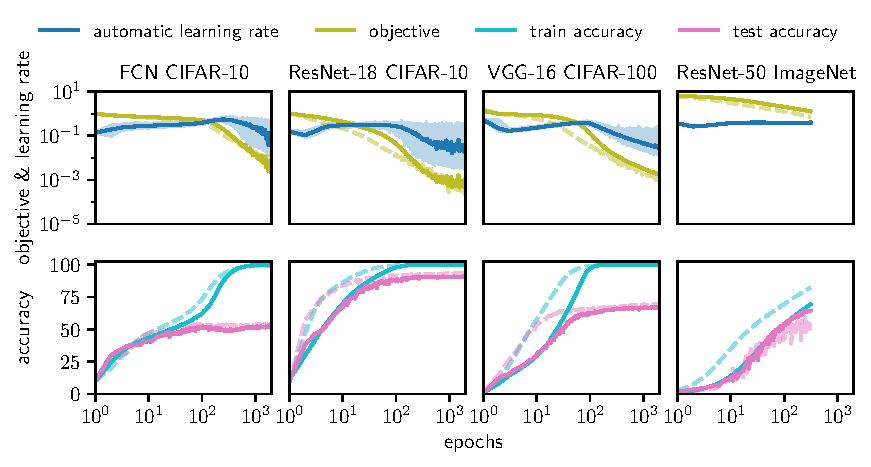
\includegraphics[width=\textwidth]{figures/pdf/plot1_full}
    \caption{\captiontitle{Benchmarking automatic gradient descent on a range of architectures and datasets.} Solid lines are AGD and faint dashed lines are tuned Adam except for ImageNet where the dashed line is SGD with a fixed learning rate of 0.1. ImageNet used cross-entropy loss with a mini-batch size of 1024. The other experiments used square loss with a mini-batch size of 128.
    The \captiontitle{top row} plots the automatic learning rate ($\eta$ in the main text) and objective value. The maximum and minimum learning rate for each epoch is included in addition to the mean for the first three plots. The \captiontitle{bottom row} shows the train and test accuracy.
    }\label{fig:1}
\end{figure}

The goal of our experiments was twofold. First, we wanted to test automatic gradient descent (AGD, \cref{alg:agd}) on a broad variety of networks architectures and datasets to check that it actually works. In particular, we tested AGD on fully-connected networks (FCNs, \cref{def:dln}), and both VGG-style \citep{simonyan2015a} and ResNet-style \citep{He2015DeepRL} convolutional neural networks on the CIFAR-10, CIFAR-100 \citep{Krizhevsky09learningmultiple} and ImageNet \citep[ILSVRC2012]{deng2009imagenet} datasets with standard data augmentation. And second, to see what AGD may have to offer beyond the status quo, we wanted to compare AGD to tuned Adam and SGD baselines, as well as Adam and SGD run with their default hyperparameters.

To get AGD working with convolutional layers, we adopted a per-submatrix normalisation scheme. Specifically, for a convolutional tensor with filters of size $\mathtt{k_x} \times \mathtt{k_y}$, we implemented the normalisation separately for each of the $\mathtt{k_x} \times \mathtt{k_y}$ submatrices of dimension $\mathtt{channels_{in}} \times \mathtt{channels_{out}}$. Since AGD does not yet support biases or affine parameters in batchnorm, we disabled these parameters in all architectures. To at least adhere to \cref{prescription:norm} at initialisation, AGD draws initial weight matrices uniform semi-orthogonal and re-scaled by a factor of $\sqrt{\mathtt{fan\_in}/\mathtt{fan\_out}}$. Adam and SGD baselines used the PyTorch default initialisation. A PyTorch implementation of AGD reflecting these details is given in \cref{app:pytorch}. All experiments use square loss except ImageNet which used cross-entropy loss. Cross-entropy loss has been found to be superior to square loss for datasets with a large number of classes \citep{Demirkaya2020ExploringTR,HuiSquareCrossEntropy}.

% We will quote the test accuracy of a model to be that of the epoch with the lowest training loss.

Our experimental results are spread across five figures:
\begin{itemize}[leftmargin=*]
    \item \cref{fig:showcase} presents some highlights of our results: First, AGD can train networks that Adam and SGD with default hyperparameters cannot. Second, for ResNet-18 on CIFAR-10, AGD attained performance comparable to the best-tuned performance of Adam and SGD. And third, AGD scales up to ImageNet.
    \item \cref{fig:1} displays the breadth of our experiments: from training a 16-layer fully-connected network on CIFAR-10 to training ResNet-50 on ImageNet. Adam's learning rate was tuned over the logarithmic grid $\{10^{-5},10^{-4},...,10^{-1}\}$ while for ImageNet we used a default learning rate of 0.1 for SGD without any manual decay. AGD and Adam performed almost equally well on the depth-16 width-512 fully-connected network: 52.7\% test accuracy for AGD compared to 53.5\% for Adam.
    For ResNet-18 on CIFAR-10, Adam attained  92.9\% test accuracy compared to AGD's 91.2\%. On this benchmark, a fully-tuned SGD with learning rate schedule, weight decay, cross-entropy loss and bias and affine parameters can attain 93.0\% test accuracy \citep{kuangliu}. For VGG-16 on CIFAR-100, AGD achieved 67.4\% test accuracy compared to Adam's 69.7\%.
    Finally, on ImageNet AGD achieved a top-1 test accuracy of 65.5\% after 350 epochs.
    \item \cref{fig:2} compares AGD to Adam and SGD for training an eight-layer fully-connected network of width 256. Adam and SGD's learning rates were tuned over the logarithmic grid $\{10^{-5},10^{-4},...,10^{-1}\}$. Adam's optimal learning rate of $10^{-4}$ was three orders of magnitude smaller than SGD's optimal learning rate of $10^{-1}$. SGD did not attain as low of an objective value as Adam or AGD.
    \item \cref{fig:3} shows that AGD can train FCNs with width ranging from 64 to 2048 and depth from 2 to 32 and \cref{fig:4} shows that AGD successfully trains a four-layer FCN at varying mini-batch size: from 32 to 4096.
\end{itemize}

\begin{figure}
    \centering
    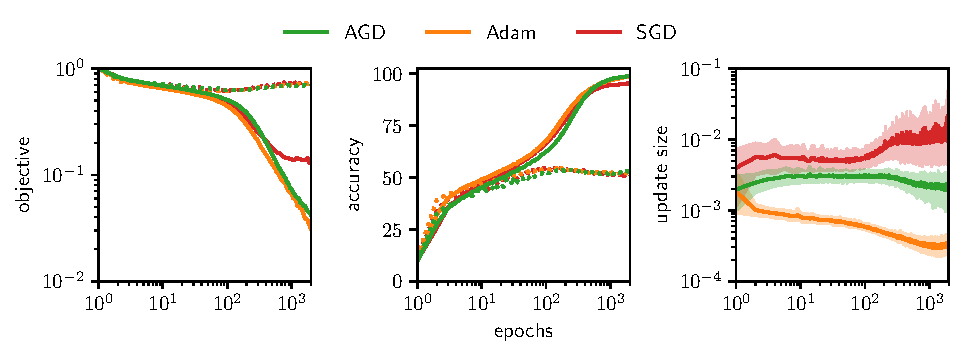
\includegraphics[width=\textwidth]{figures/pdf/plot2}
    \caption{\captiontitle{Comparing automatic gradient descent to tuned Adam and SGD.} An eight-layer fully-connected network was trained on CIFAR-10 with square loss. Dotted lines show test and solid lines show train performance.
    The \captiontitle{left panel} shows the objective value: AGD and Adam attained a smaller training objective than SGD. The \captiontitle{middle panel} shows train and test accuracies. The \captiontitle{right panel} shows the relative update size averaged over layers: $\tfrac{1}{L}\sum_{k=1}^L \norm{\Delta \mW_k}_F/\norm{\mW_k}_F$. We plot the maximum, minimum and mean over an epoch.} \label{fig:2}
\end{figure}
\begin{figure}
    \centering
    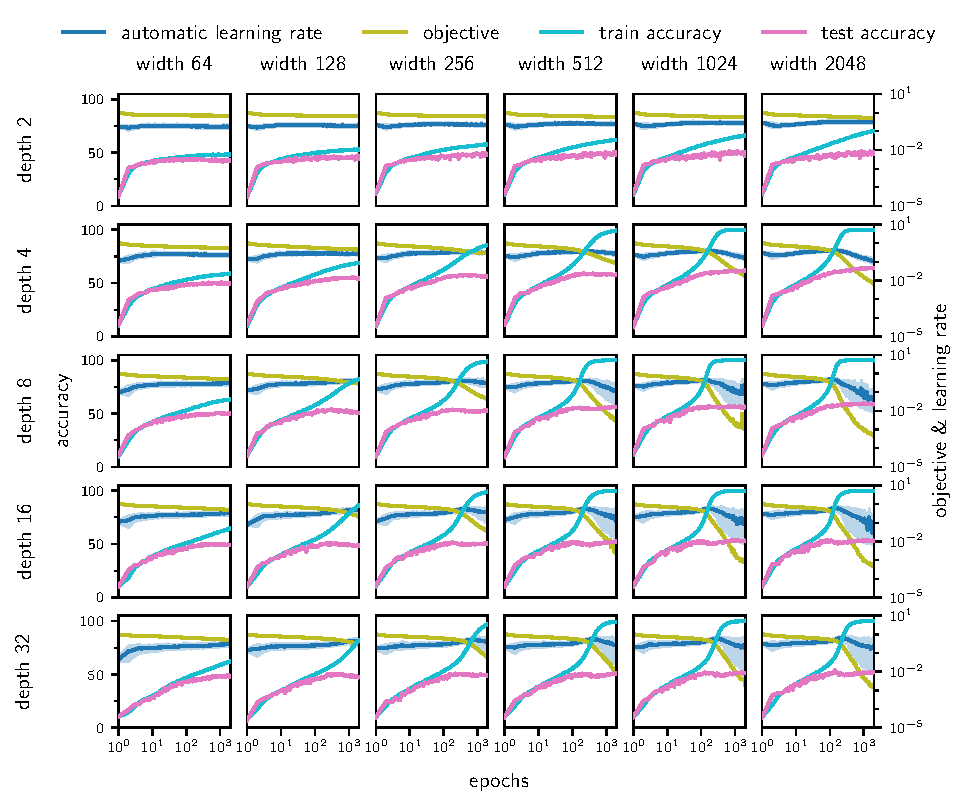
\includegraphics[width=\textwidth]{figures/pdf/plots3_0}
    \caption{\captiontitle{Benchmarking automatic gradient descent on networks of varying width and depth.} We trained fully-connected networks on CIFAR-10 with square loss and a mini-batch size of 128. The depth ranged from $2$ to $32$, and the width from $64$ to $2048$, in powers of two. In terms of training performance, wider was always better, while depth 8 and depth 16 were superior to depth 32. In terms of test accuracy, the best performance was achieved at depth 4 and width 2048: 63.7\%. The worst test performance was achieved by the smallest network of depth 2 and width 64: 42.55\%.
    Larger networks display two broadly distinct phases of training: the automatic learning rate increases slowly while the objective decreases slowly, followed by a rapid decrease in the automatic learning rate and objective. This second phase typically coincides with reaching 100\% train accuracy. See \cref{fig:2} for a comparison between Adam, SGD and AGD for the 256-width 8-layer FCN.} \label{fig:3}
\end{figure}
\begin{figure}
    \centering
    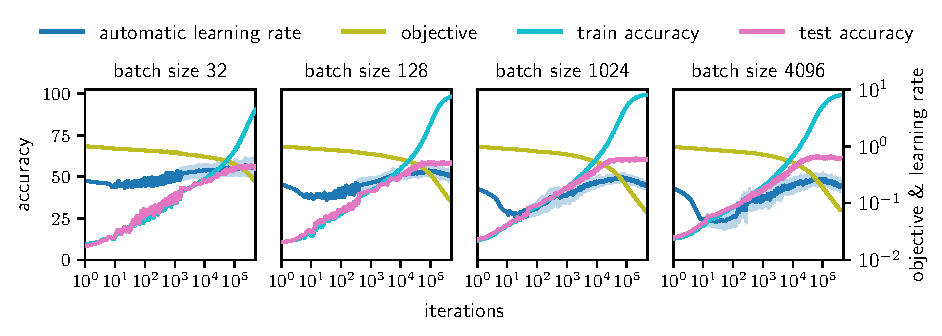
\includegraphics[width=\textwidth]{figures/pdf/plot4}
    \caption{\captiontitle{Benchmarking automatic gradient descent at varying mini-batch size.} We trained four-layer fully-connected networks on CIFAR-10. The mini-batch size ranged from 32 to 4096. Test accuracy generally improved with increasing mini-batch size: the final test accuracies, in order of increasing mini-batch size, were 55.0\%, 58.0\%, 60.0\% and 59.8\%. The automatic learning rate seemed to initially dip, and this effect was more pronounced for larger mini-batch sizes. Metrics were computed every iteration during the first epoch and once per epoch from thereon---this explains the kinks visible in the plots.
    } \label{fig:4}
\end{figure}
